\addcontentsline{toc}{section}{Results}
\section*{Results}
\label{sec:Results}

All the necessary concepts in the theory for the model have been covered,
so we are free to fully discuss the computational portion.

\addcontentsline{toc}{subsection}{Verifying Implementation}
\subsection*{Verifying Implementation}
\label{subsec:verify}

Before we invesigate the results of the computational modeling, we gain
confidence in the correctness of the programs by checking values over time.
We also use autocorrelation to further support the correctness of the
propagation.

\addcontentsline{toc}{subsubsection}{Examining Expected Values}
\subsubsection*{Examining Expected Values}

First, we check if my implemetned operator is unitary. For all graphs, the
$x$-axis is displaying time unless specified otherwise. The final time is
fixed.

\begin{figure}[H]
    \centering
    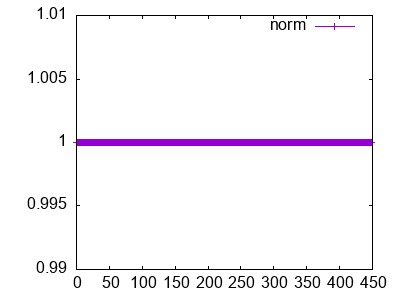
\includegraphics[width=0.6\textwidth]{norm.png}
    \caption[Squared Magnitude of the Wave Function over Time]{The
    \texttt{norm} axis indicates the sum of all the elements of
    $\vec{\Psi}(t)$.}
\end{figure}

The norm is one through all our time steps, so the implemented operator is
unitary, as we calculated. Now we examine the expected total energy,
momentum, and position for different $k$ values for a system with a constant
potential function and a potential well.

\pagebreak

\begin{center}
    \textit{Constant Potential}
\end{center}

We check to see if $\langle H \rangle \approx \frac{k^2}{2}$ and $\left|
\frac{d}{dt} \langle x \rangle \right| = \left| \langle p \rangle \right|
\approx k$, and that they behave roughly as explained in the
\nameref{sec:expected} section.

For $k = 0.59$, I computed with the programs
the following values.

\begin{figure}[H]
    \centering
    \begin{tabular}{cc}
        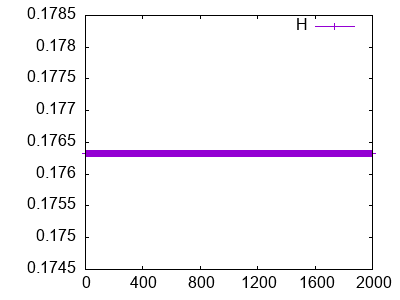
\includegraphics[width=0.4\textwidth]{Hc0.59.png}
        &
        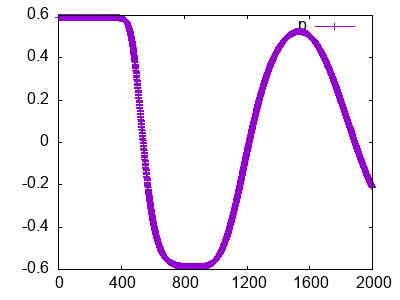
\includegraphics[width=0.4\textwidth]{pc0.59.png}
        \\
        (a) & (b)
        \\
        \multicolumn{2}{c}
        {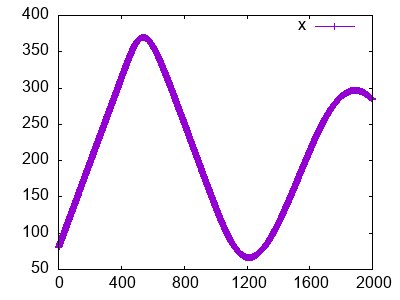
\includegraphics[width=0.4\textwidth]{xc0.59.png}}
        \\
        \multicolumn{2}{c}{(c)}
    \end{tabular}
    \caption[Expected Values over Time for $k = 0.59$]{The three plots
    display the expected values over time for $k = 0.59$. The $y$-axis in
    plot (a) indicates the total energy of the system. The $y$-axis in plots
    (b) and (c) indicate the expected momentum and expected position of the
    wave packet, respectively.}
    \label{fig:c0.59}
\end{figure}

The value $\frac{d}{dt} \langle x \rangle$ is equal to the slope in plot (c)
in Figure \ref{fig:c0.59}, which can be computed using the coorindates
$(x, t) = (0, 80), (81, 127.34)$ from the datafile: $\frac{d}{dt} \langle x
\rangle \approx 0.58 \approx k$. The computational expectation values for
the total energy of the system and momentum of the wave packet are
consistent with the theory.

\pagebreak

Now for $k = 1$, the programs output the following data.

\begin{figure}[H]
    \centering
    \begin{tabular}{cc}
        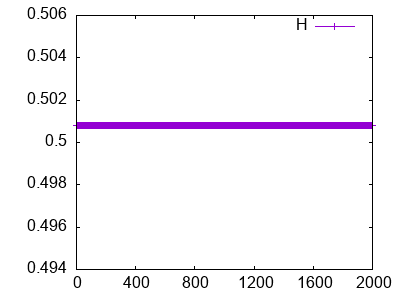
\includegraphics[width=0.4\textwidth]{Hc1.png}
        &
        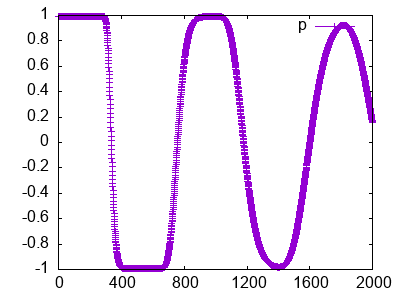
\includegraphics[width=0.4\textwidth]{pc1.png}
        \\
        (a) & (b)
        \\
        \multicolumn{2}{c}{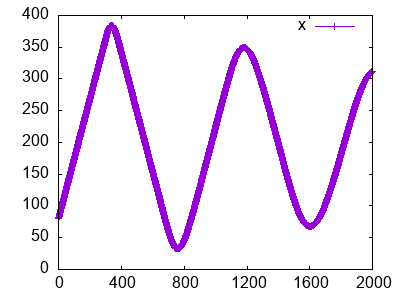
\includegraphics[width=0.4\textwidth]{xc1.png}}
        \\
        \multicolumn{2}{c}{(c)}
    \end{tabular}
    \caption[Expected Values over Time for $k = 1$]{The three plots display
    the expected values over time for $k = 1$. The $y$-axis in plot (a)
    indicates the total energy of the system. The $y$-axis in plots (b) and
    (c) indicate the expected momentum and expected position of the wave
    packet, respectively.}
    \label{fig:c1}
\end{figure}

The value $\frac{d}{dt} \langle x \rangle$ is equal to the slope in plot (c)
in Figure \ref{fig:c1}, which can be computed using the coorindates $(x, t)
= (0, 80), (81, 156.43)$ from the datafile: $\frac{d}{dt} \langle x \rangle
\approx 0.94 \approx k$. The wave packet moves over more distance in the
same amount of time for a larger $k$. The computational expectation values
are consistent with the theory.

\pagebreak

\begin{center}
    \textit{Finite Potential Square Well}
\end{center}

I used the following potential well.

\begin{figure}[H]
    \centering
    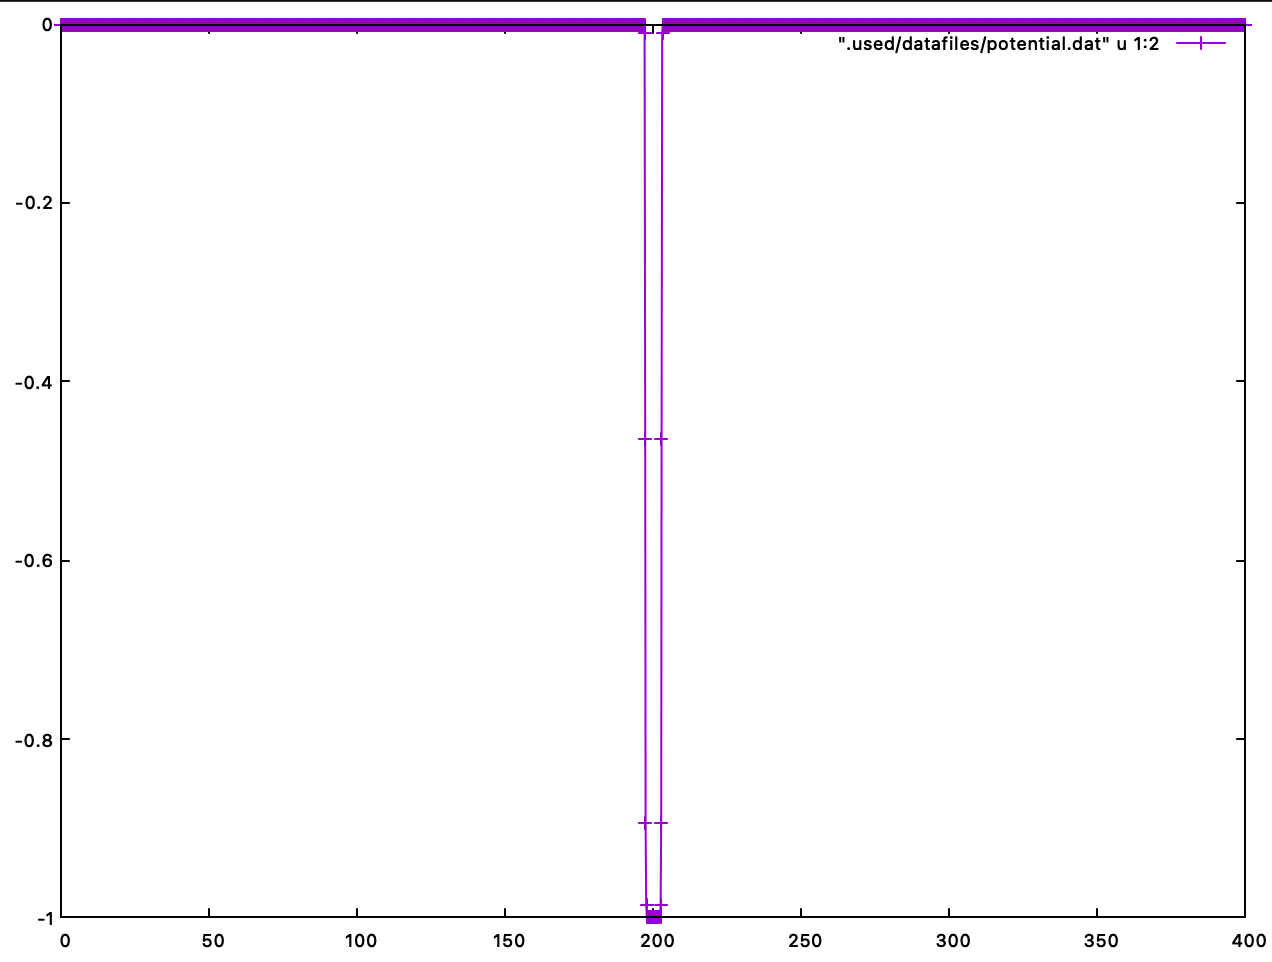
\includegraphics[width=0.6\textwidth]{smallwell.png}
    \caption[Small Potential Well]{The $y$-axis represents the potential
    energy, and the $x$-axis represents the position within the box.}
    \label{fig:smallwell}
\end{figure}

We check to see if $\langle H \rangle \approx \frac{k^2}{2}$ and if
initially $\left| \frac{d}{dt} \langle x \rangle \right| = \left| \langle p
\rangle \right| \approx k$, and that they behave roughly as explained in the
\nameref{sec:expected} section. The width of the well used was $0.01R$, and
the full width at half maximum (FWHM) of the Gaussian scalar function of the
initial wave packet used is $20\sqrt{2\log(2)}$ in $x$ space.

Figure \ref{fig:w} on the next page shows the numerical computations of the
expected value of each of the physical quantities for $k = 0.59, 1$, as
calculated by the programs.

\begin{figure}[H]
    \centering
    \begin{tabular}{ccc}
        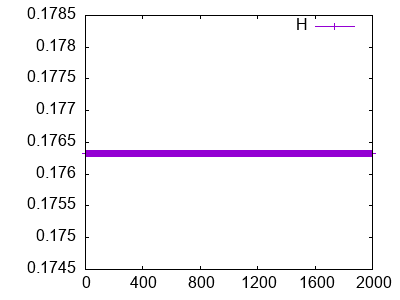
\includegraphics[width=0.3\textwidth]{Hw0.59.png}
        &
        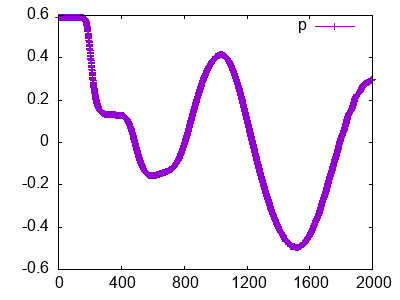
\includegraphics[width=0.3\textwidth]{pw0.59.png}
        &
        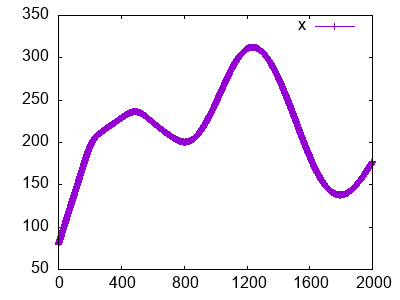
\includegraphics[width=0.3\textwidth]{xw0.59.png}
        \\
        (a) & (b) & (c)
        \\
        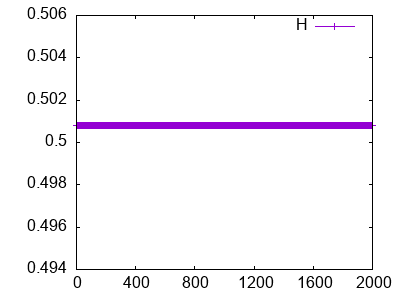
\includegraphics[width=0.3\textwidth]{Hw1.png}
        &
        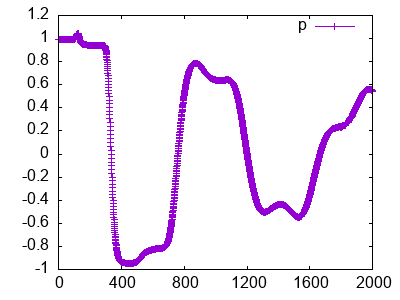
\includegraphics[width=0.3\textwidth]{pw1.png}
        &
        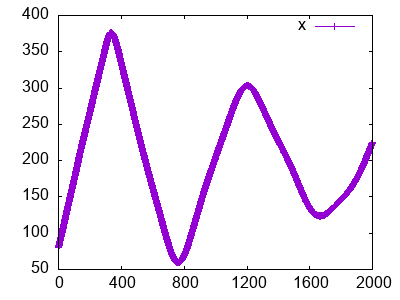
\includegraphics[width=0.3\textwidth]{xw1.png}
        \\
        (d) & (e) & (f)
    \end{tabular}
    \caption[Expected Values for a Large Well for $k = 0.59, 1$]{The top
    three plots display the expected values over time for
    $k = 0.59$, and the bottom three for $k = 1$. The $y$-axis in plots (a)
    and (d) indicates the total energy of the system. The $y$-axis in plots
    (b) and (e) indicates the expected momentum, and the $y$-axis in plots
    (c) and (f) indicates the expected position of the wave packet.}
    \label{fig:w}
\end{figure}

Although we will not compute the initial slope of plots (c) and (f), we may
notice that the predicted change in the expected position is represented in
the graphs, so the computational expected values are consistent with the
theory. The discrepancies between the graphs for $k = 0.59$ and $k = 1$ will
be discussed in further detail in the \nameref{subsec:num} subsection.

\addcontentsline{toc}{subsubsection}{Autocorrelation for $\left| \Psi
\right| ^ 2$ through Negative Time}
\subsubsection*{Autocorrelation for $\left| \Psi \right| ^ 2$ through
Negative Time}

We assess correctness with autocorrelation by checking if it is
approximately equal to one.  The following is the schema for measuring
autocorrelation, where $n \in \mathbb{Z}$.

\begin{align*}
    \Psi(n \delta t) &=
    \left(
    \frac{1 - iH\frac{\delta t}{2}}{1 + iH\frac{\delta t}{2}}
    \right)^n
    \Psi(0)
    \\
    {\tilde{\Psi}}_n(0) &=
    \left(
    \frac{1 - iH\frac{-\delta t}{2}}{1 + iH\frac{-\delta t}{2}}
    \right)^n
    \Psi(n \delta t)
    \\
    \mathrm{autocorrelation} &=
    \int_0^R \Psi(0)^* \tilde{\Psi}(0) dx
\end{align*}

To implement this measure using the implicit scheme of propagation, I
propagated forward in time by $n$ time steps, and backward in time by the
same number of time steps. The integral was calculated by summing the
product of each element of $\vec{\Psi}(0)$ and the complex conjugate of its
corresponding element of $\vec{\tilde{\Psi}}(0)$.

\begin{figure}[H]
    \centering
    
\includegraphics[width=0.7\textwidth]{autocorr.out.png}
    \caption[Autocorrelation output]{The output for the autocorrelation for
    $\delta t = 0.9$ and the $n = 2222$.}
\end{figure}

The autocorrelation is exactly equal to one because the error in forward
propagation is equal to the negative of the backward negative operator
because a factor of the propagator error, $\delta t^3$, is odd with respect
to $\delta t$.

\addcontentsline{toc}{subsection}{Numerical Calculations of the Transmission
Coefficient}
\subsection*{Numerical Calculations of the Transmission Coefficient}
\label{subsec:num}

I numerically calculated the transmission coefficient by

\[
    \sum_{j = A}^N \vec{\Psi}_j(t_f)
\]

where $A$ is the number of spacial steps that corresponds to the approximate
edge of the well that is on the side opposite of the starting position of
the wave packet, $N$ is again the total number of spacial steps. This
summation is computed at $t_f$, corresponding to a time after the full
transmission through the well has occured.

\begin{figure}[H]
    \centering
    \begin{tabular}{cc}
        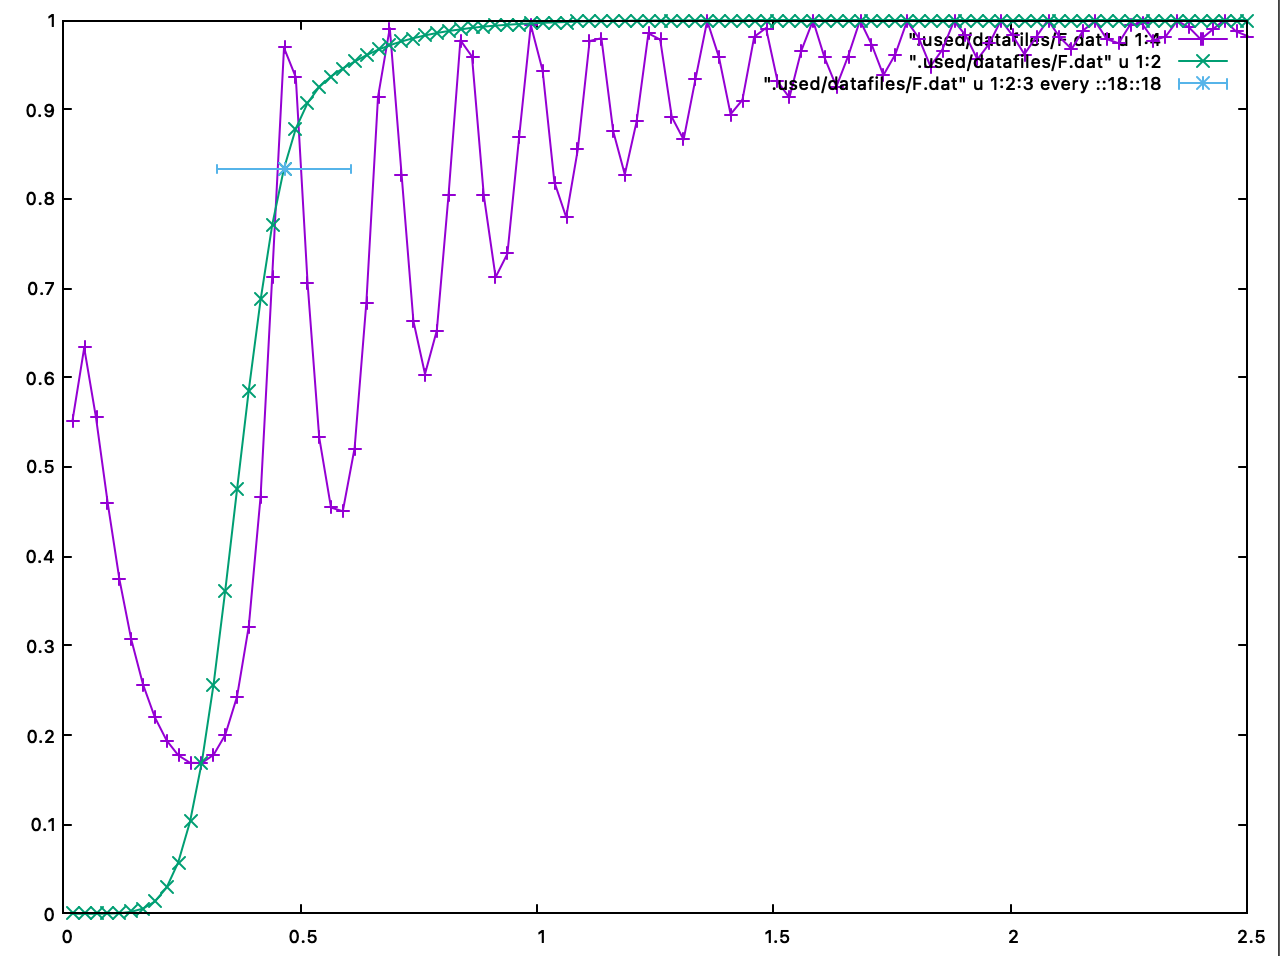
\includegraphics[width=0.4\textwidth]{translarge.png}
        &
        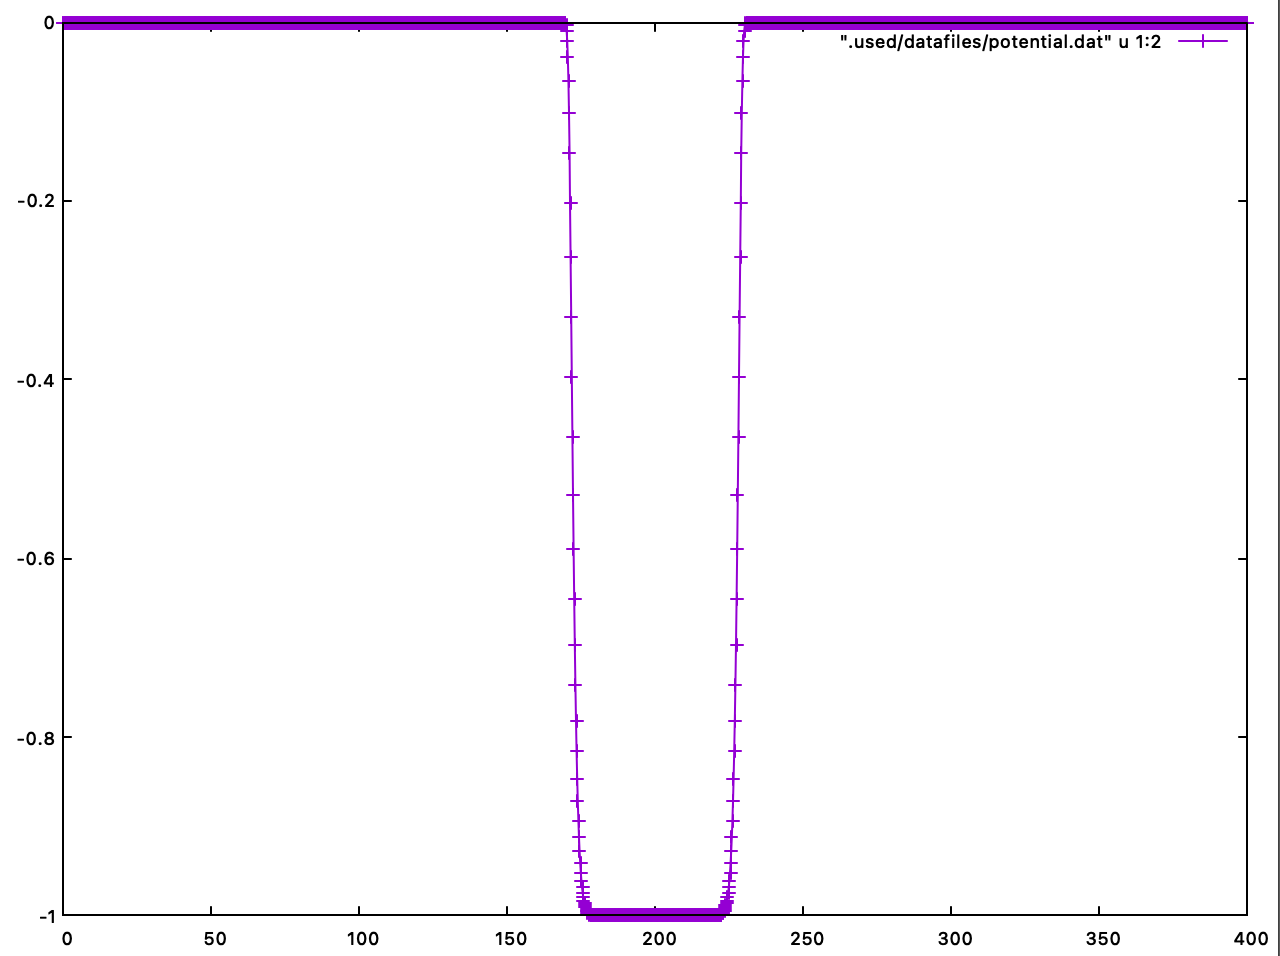
\includegraphics[width=0.4\textwidth]{largewell.png}
        \\
        (a) & (b)
    \end{tabular}
    \caption[Large Well Transmission]{The $x$-axis represents $k$. The
    transmission coefficient as calculated analytically is plotted in purple
    and as computed numerically is plotted in turquoise. The length of each
    side of the error bar is the half width of the wave packet in $k$ space,
    calculated by $\frac{2}{\sqrt{2\sigma^2}}$ where $\sigma$ is the
    standard deviation parameter for the Gaussian envelope.}
    \label{translarge}
\end{figure}

We see that the numerical computation does not match the analytical solution.
If we recall that the analytical solution is for an eigenstate, and that a
wave packet is superposition of many eigenstates, it is then reasonable to
guess that the plot of the numerical solution appears as sort of an
$S$-curve because the transmission of all plane waves composing the wave
packet, each of which corresponds to its own $k$ value, are summed, and that
the center of the $k$ distribution is larger than one oscillation in the
analytical solution. We must reduce the width of the wave packet in
$k$-space in order for the numerical plot to resemble the analytical plot.
This corresponds to a decrease in the width of the wave packet in $x$-space,
which at this point we may reduce the width of the well to maintain an
approximately infinitely large box\footnote[1]{The relation between the well
width in $x$-space and $k$-space is calculated by Fourier transform and
FWHM of the wave packet.}. The graph (a) in Figure \ref{translarge} uses a
well width of $0.1R$, seen in graph (b). The following figure uses a well
width of $0.01R$, seen in Figure \ref{fig:smallwell}.

\begin{figure}[H]
    \centering
    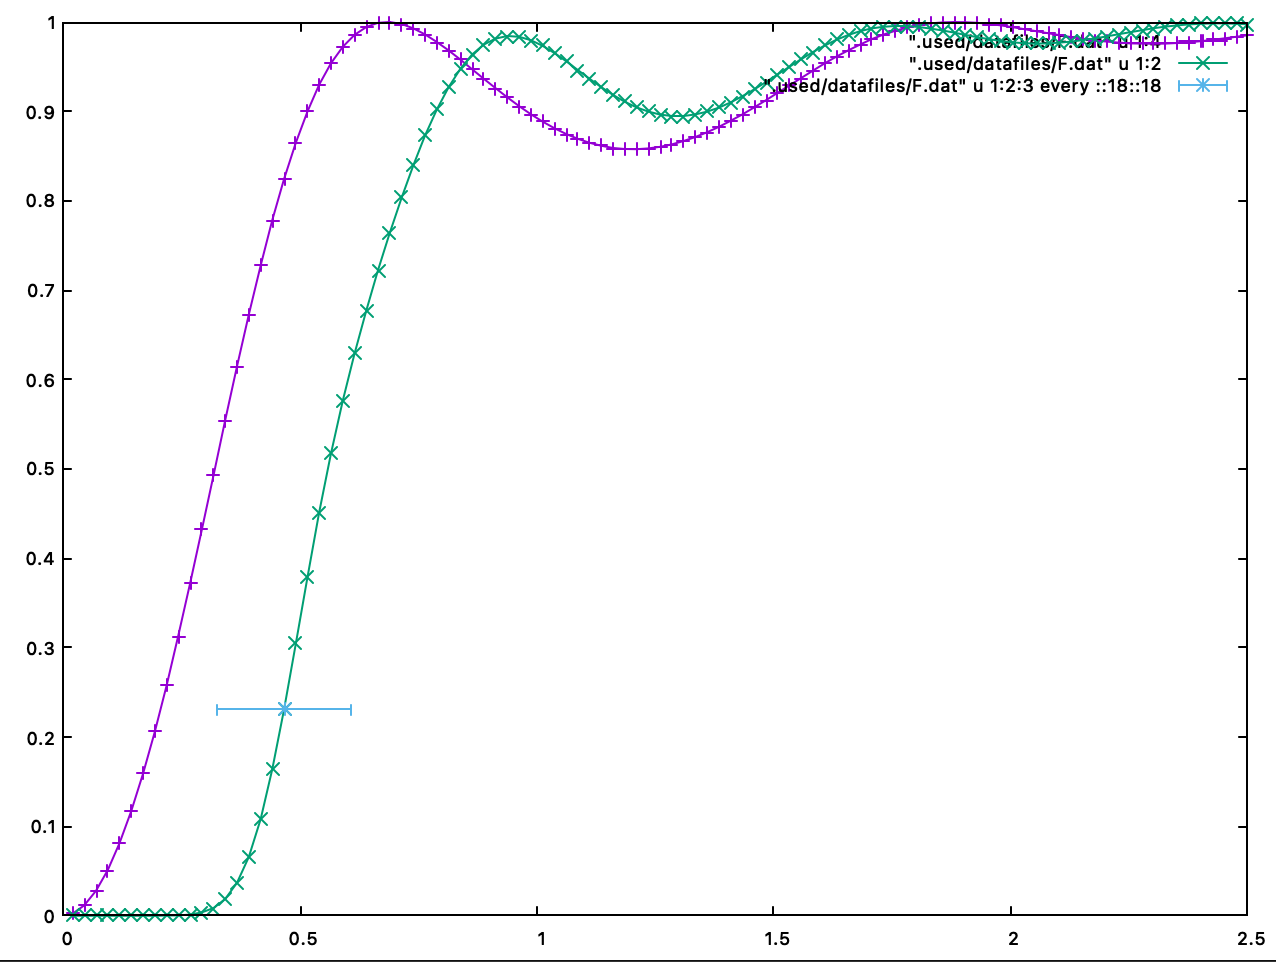
\includegraphics[width=0.6\textwidth]{transsmall.png}
    \caption[Small Well Transmission]{The plots are the same as in Figure
    \ref{translarge}.}
\end{figure}

We see now that the error bar is smaller than one oscillation in the
analytical plot, and that both functions match with an offset of some phase
constant.

Revisiting the graphs for the expected values over time for a system with a
finite potential well (Figure \ref{fig:w}), we noted the differences in the
expected values over $k = 0.59$ and $k = 1$. If we compare those to the
graphs in Figures \ref{fig:c0.59} and \ref{fig:c1}, we see that the expected
values behave more similarly between a constant potential and a potential
well for $k = 1$ than $k = 0.59$. This is because there is a larger
transmission at $k = 0.59$, which is supported by the analytical plot.

\addcontentsline{toc}{subsubsection}{Extended Verification}
\subsubsection*{Extended Verification}

We extend our verification process by examining the wave packet and
transmission over time over $k$. We notice a reflection and transmission in
Figure \ref{fig:wellanim}, and an oscillation in transmission (equal to the
plateau since the initial wave packet is normalized) through $k$ in Figure
\ref{fig:Fanim}.

\begin{figure}[H]
    \centering
    \begin{tabular}{cc}
        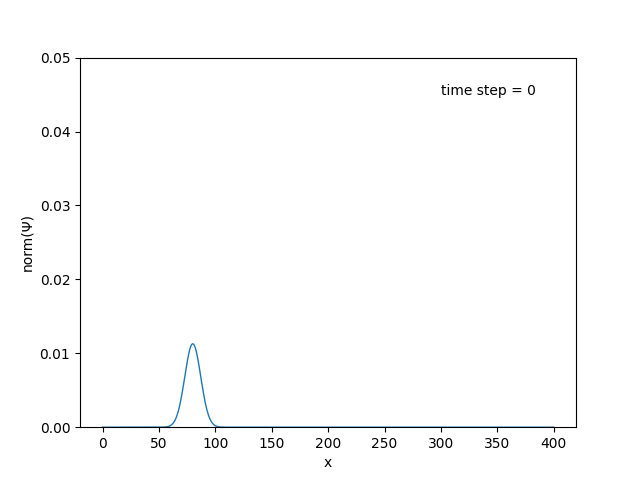
\includegraphics[width=0.4\textwidth]{well1.png}
        &
        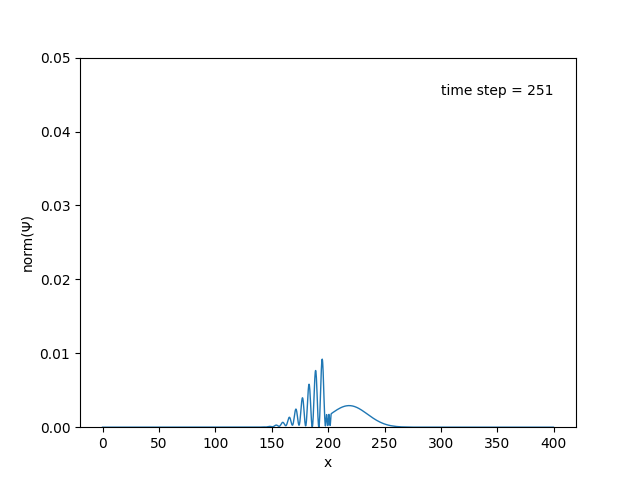
\includegraphics[width=0.4\textwidth]{well252.png}
        \\
        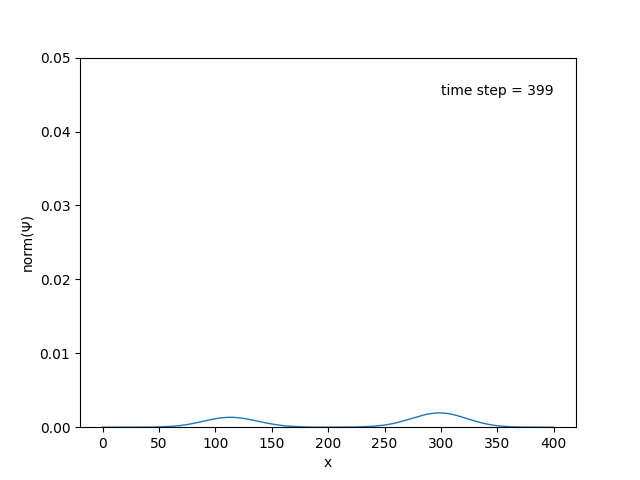
\includegraphics[width=0.4\textwidth]{well400.png}
        &
        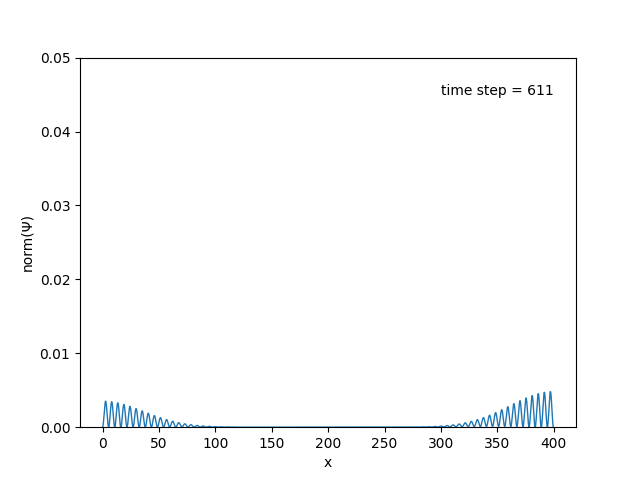
\includegraphics[width=0.4\textwidth]{well612.png}
    \end{tabular}
    \caption[Well Propagation]{The square magnitude of the wave packet at
    four different time steps}
    \label{fig:wellanim}
\end{figure}

\begin{figure}[H]
    \centering
    \begin{tabular}{ccc}
        \includegraphics[width=0.3\textwidth]{F10.png}
        &
        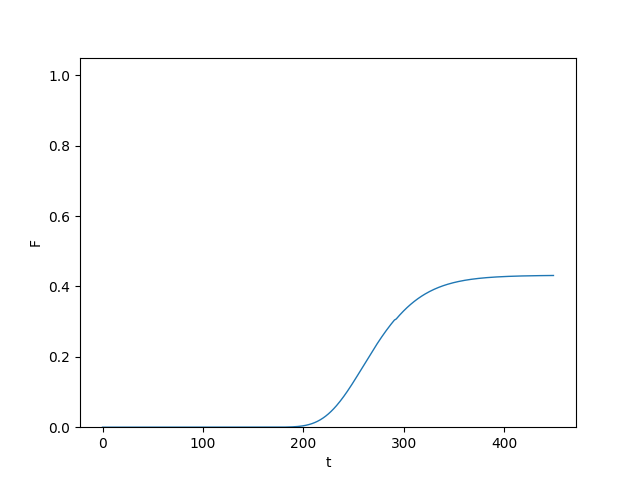
\includegraphics[width=0.3\textwidth]{F20.png}
        &
        \includegraphics[width=0.3\textwidth]{F46.png}
    \end{tabular}
    \begin{tabular}{cc}
        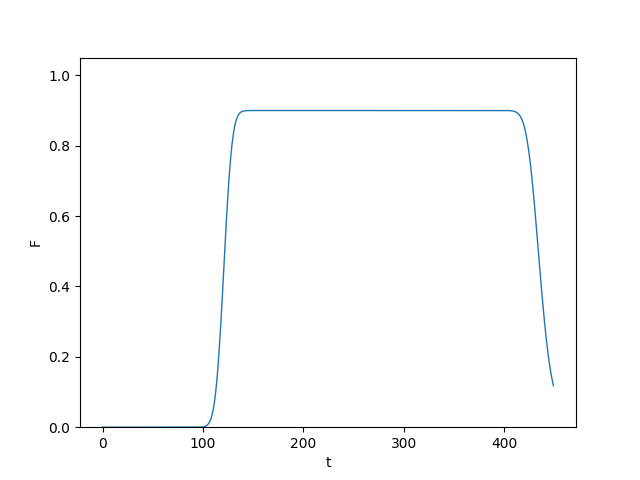
\includegraphics[width=0.3\textwidth]{F55.png}
        &
        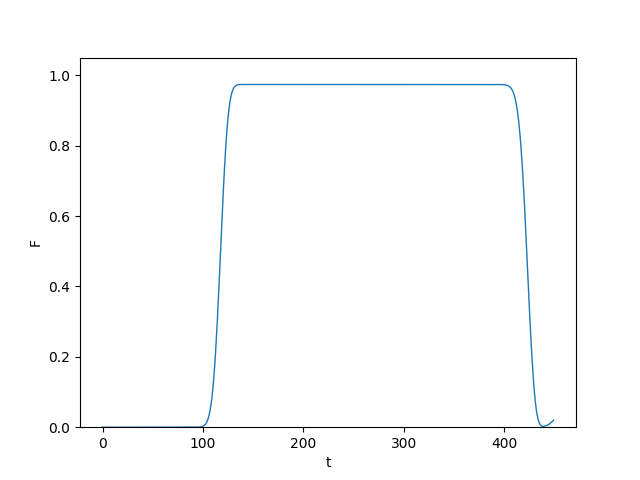
\includegraphics[width=0.3\textwidth]{F65.png}
    \end{tabular}
    \caption[Transmission Probabilities]{The probability of the localized
    particle being transmitted ($F$) over time for increasing $k$}
    \label{fig:Fanim}
\end{figure}
